\section{Carrier Detector (Morten og David)}
For at sikre at alle dele af kredsløbet fungerer, deles det op i mindre blokke, og implementeres på fumlebræt.\\
\\
Først realiseres båndpasfilteret for at konstatere, at $18 VAC 50 Hz$ delen er dæmpet, men $120 kHz$ signalet fortsat er til stede.

\begin{figure}[h]
	\centering
	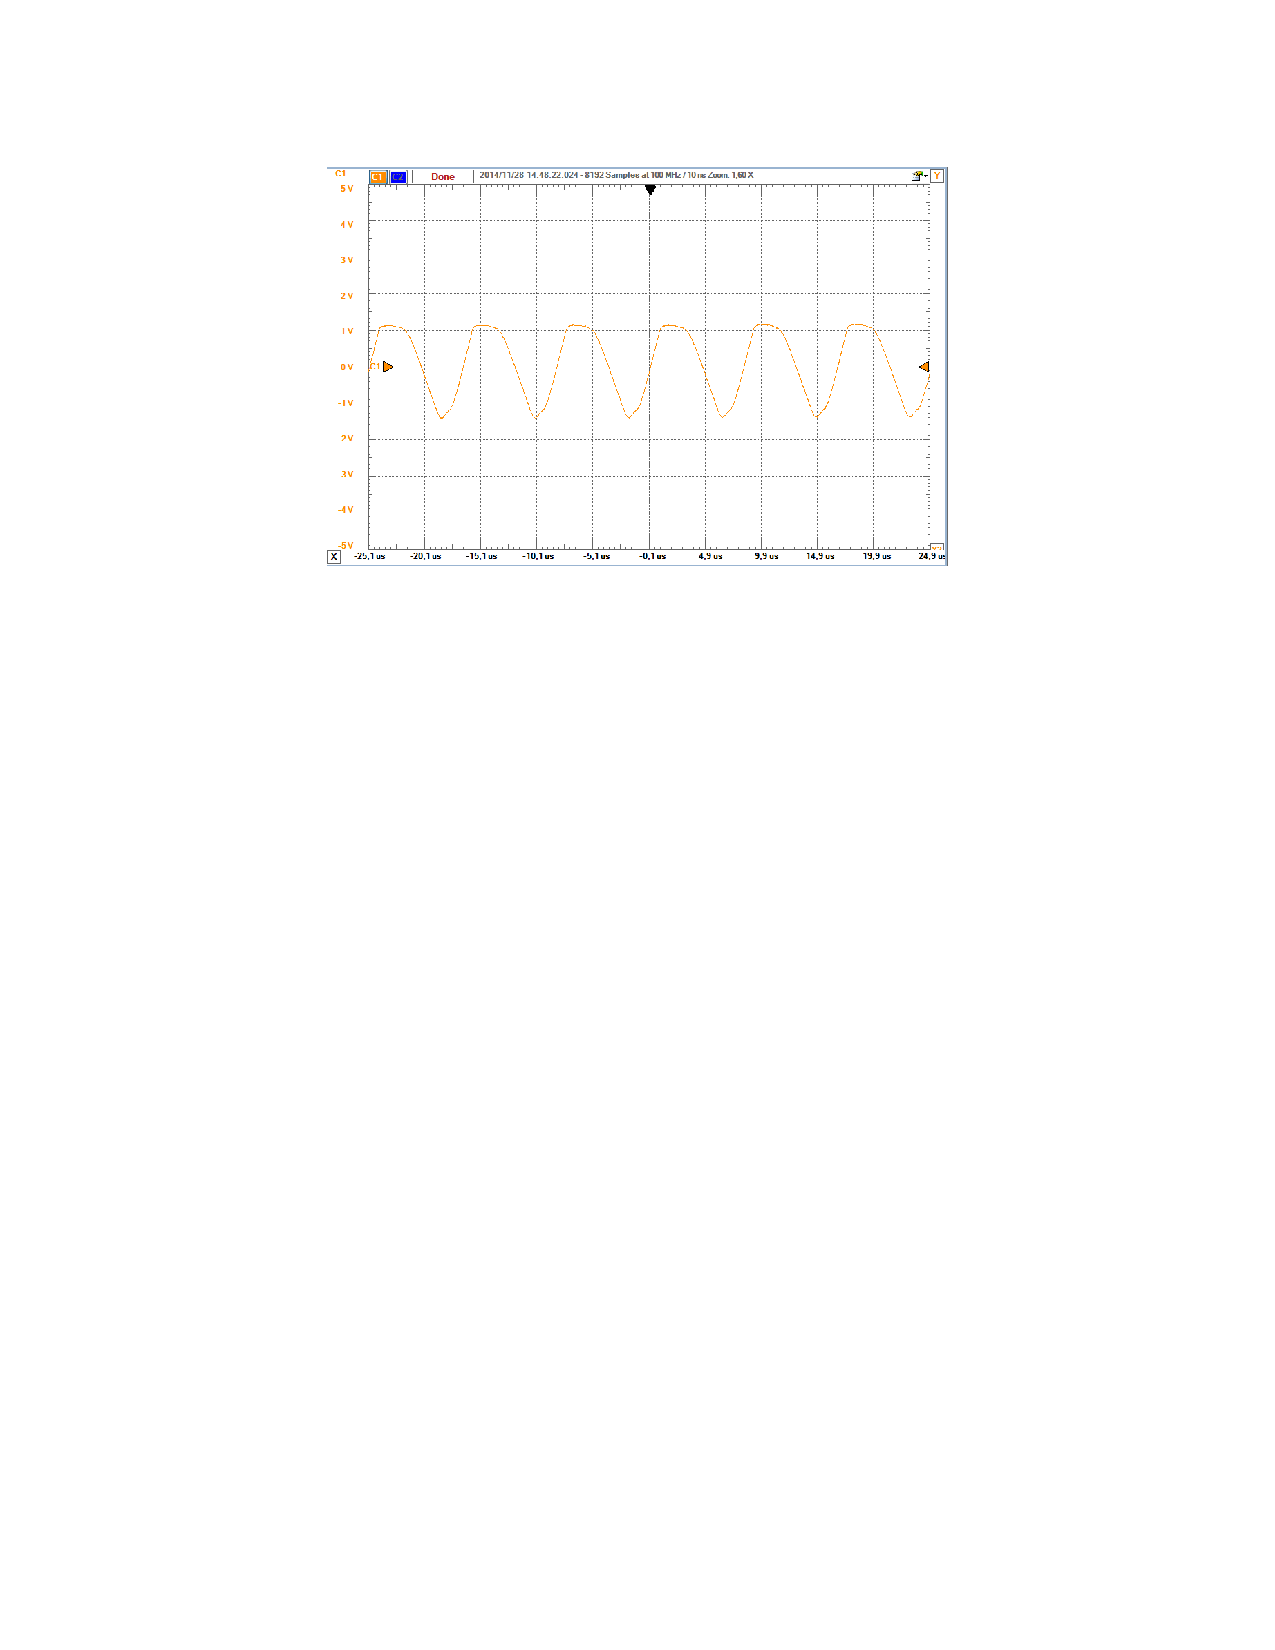
\includegraphics[width={\textwidth},trim=150 520 150 80, clip=true]{../Implementering/billeder/efter_baandpas.pdf}
	\caption{Signal efter båndpas}
	\label{fig:CD_efter_baandpas}
\end{figure}

Det ses på Figur \ref{fig:CD_efter_baandpas}, at båndpasfilteret virker som forventet. $18 VAC$ $50 Hz$ signalet er væk. $120 kHz$ signalet ser noget anderledes ud, men det har ingen betydning.\\
\\
Herefter realiseres selve envelope detektoren ($D_{5}$\cite{lib:1N4148}, $R_{11}$ og $C_{9}$), og der måles med oscilloskopet på udgangen. Signalet er vist på Figur \ref{fig:CD_efter_envelope}.

\begin{figure}[h]
	\centering
	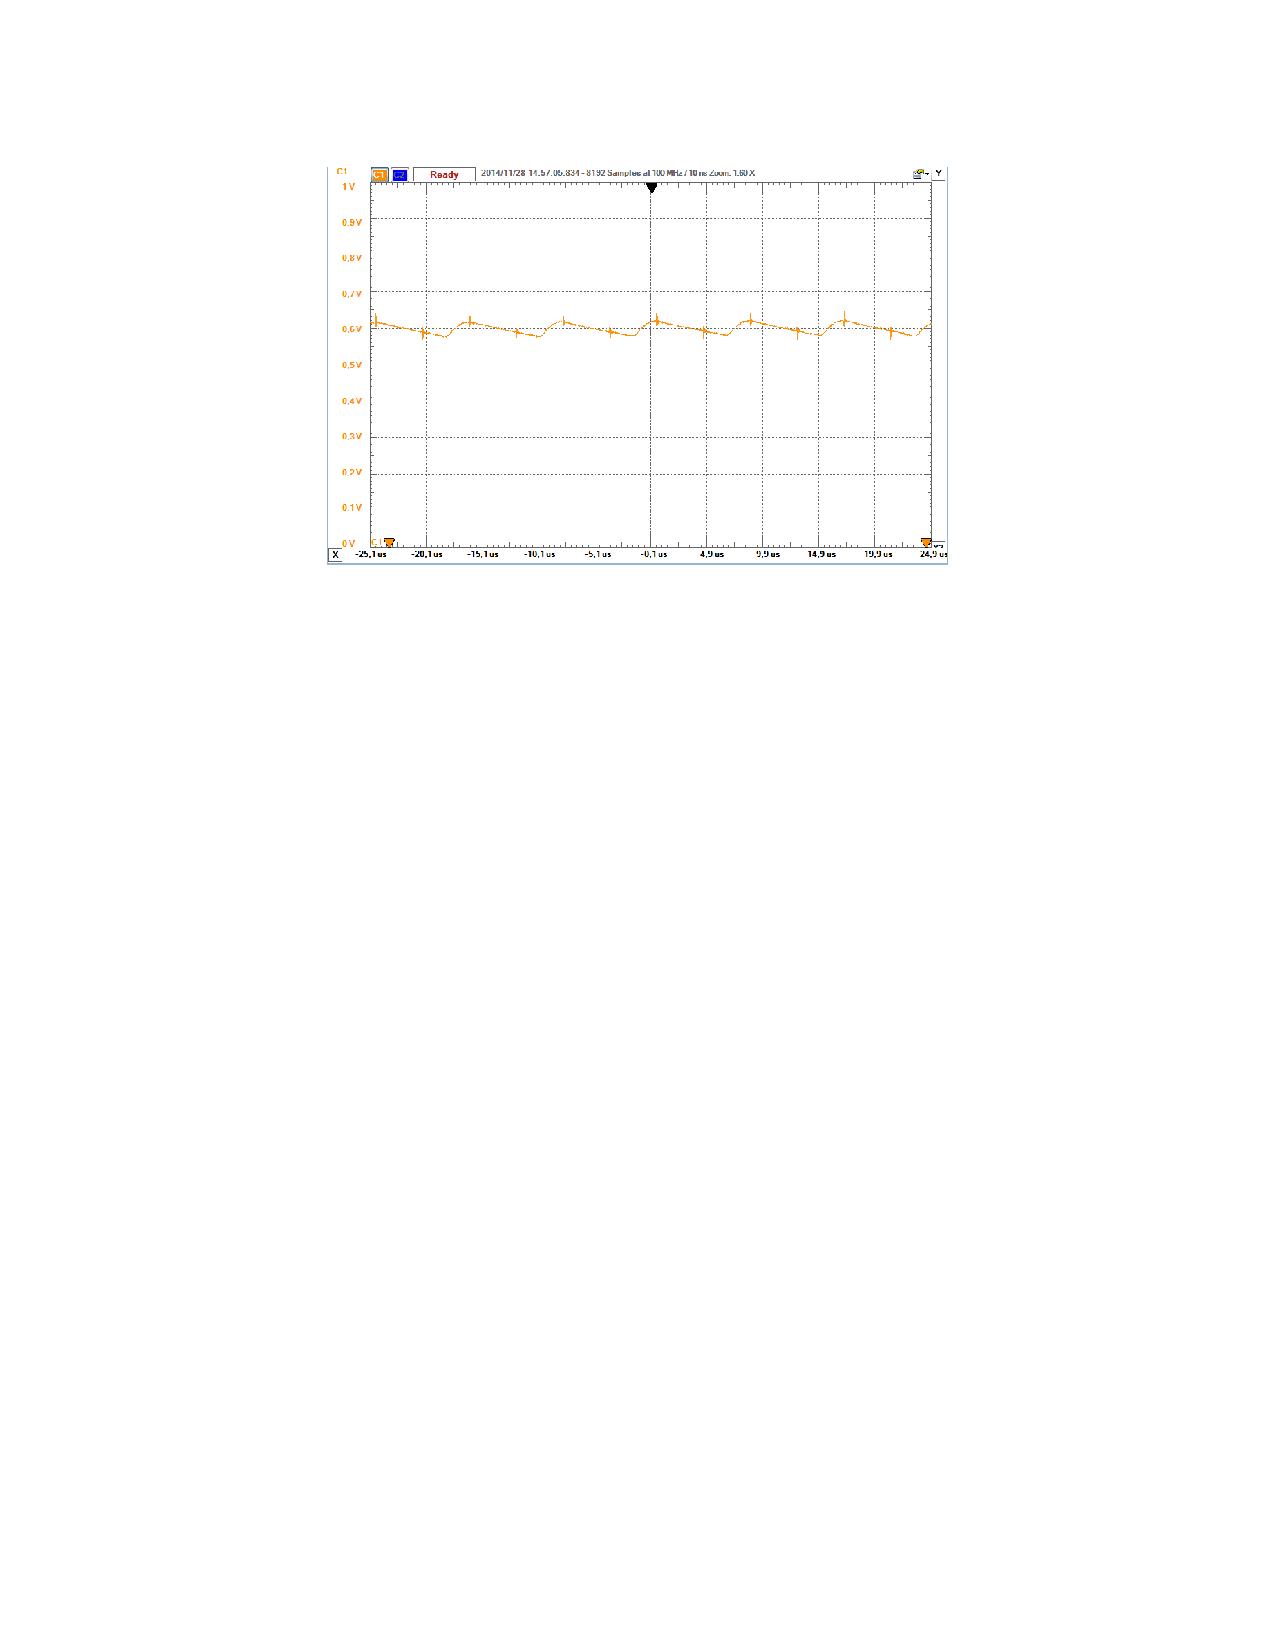
\includegraphics[width={\textwidth},trim=158 520 150 80, clip=true]{../Implementering/billeder/efter_envelope.pdf}
	\caption{Signal efter envelope detector med $120 kHz$}
	\label{fig:CD_efter_envelope}
\end{figure}
\newpage
Det ses på Figur \ref{fig:CD_efter_envelope}, envelopedetektoren fungerer. $120 kHz$ signalet ses tydeligt på takkede signal, og man kan desuden se at forholdet mellem $R_{11}$ og $C_{9}$ er passende; afladningstiden er lang nok. Det testedes desuden at udgangen på envelope detektoren gik til $0V$, når $120 kHz$ signalet fjernes.\\
\\
Signalet efter envelope detektoren ligger mellem $480 mV$ og $600 mV$, og den efterfølgende komparator \cite{lib:TS912} har derfor en reference på $318 mV$ på den inverterende indgang. Komparatoren $U_{4B}$ og dioden $D_{6}$ samt pull-down modstanden $R_{14}$ realiseres på fumlebrættet, og spændingen på udgangen måles. Uden detektion af $120 kHz$ signal måles $0.0V$ og med detektion af $120 kHz$ signal måles $4.7 V$, hvilket ligger inden for tolerancen jf. signalbeskrivelsen.\\
\\
For at sikre at rise time på bitstream er hurtig nok, måles dette med oscilloskopet; resultatet ses på Figur \ref{fig:CD_bitstream}.
 
\begin{figure}[h]
	\centering
	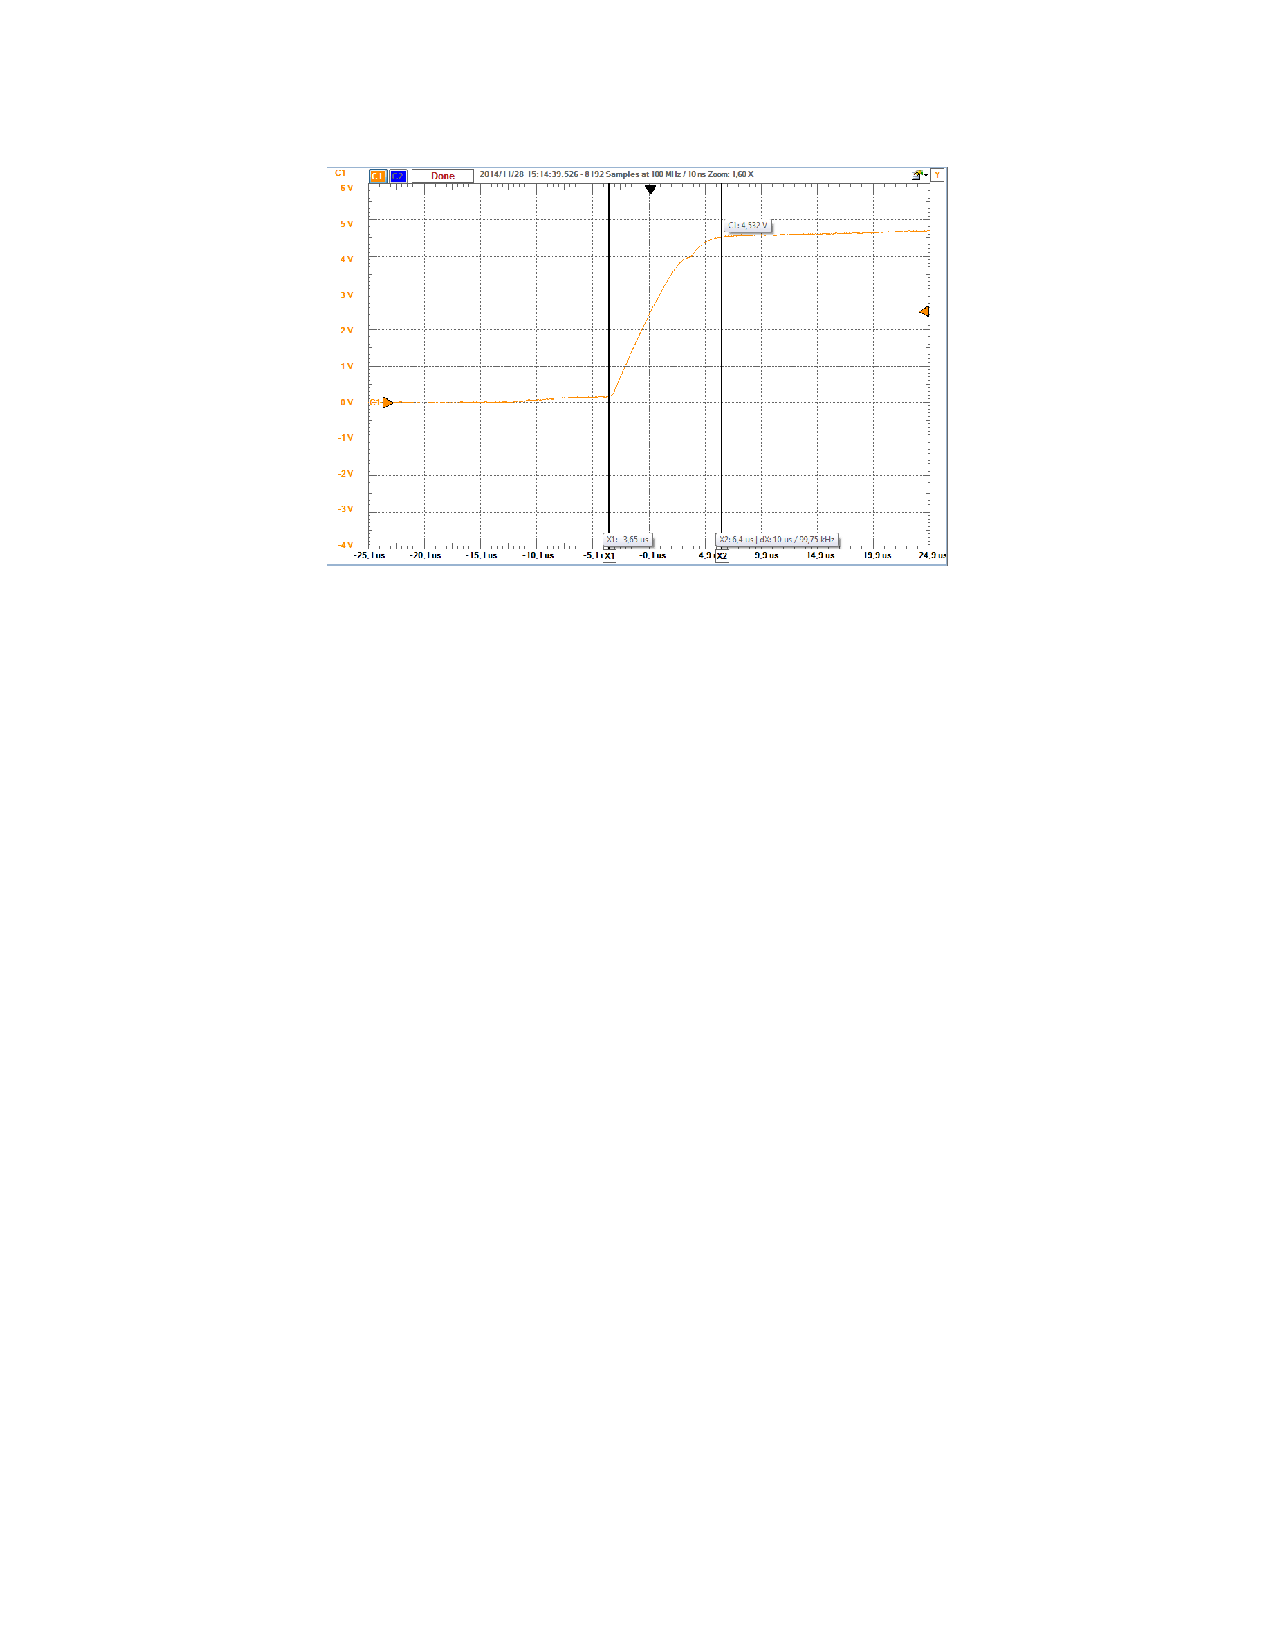
\includegraphics[width={\textwidth},trim=150 520 150 80, clip=true]{../Implementering/billeder/bitstream.pdf}
	\caption{Rising edge på bitstream}
	\label{fig:CD_bitstream}
\end{figure}
\newpage
Det ses på Figur \ref{fig:CD_bitstream}, at signalet er ca. $10 \mu s$ om gå fra lav til høj, hvilket er tilfredsstillende. Det ses desuden, at der ikke er prel på signalet.\\